\documentclass[a4paper]{article}

\usepackage[english]{babel}
\usepackage[utf8]{inputenc}
\usepackage{amsmath}
\usepackage{graphicx}
\usepackage[colorinlistoftodos]{todonotes}
\usepackage{pgfplots} % https://sv.sharelatex.com/learn/Pgfplots_package#!#Plotting_from_data

\usepackage{color}

\pgfplotsset{width=10cm,compat=1.9}

\title{Conclusions}

\author{John-John Markstedt}

\date{\today}

\begin{document}
	\maketitle
	
	This is part af a collection of yearly reports and their conclusions from 2015 forward. Here I summarize all quantitative aspects of live with the purpose to get a clear understanding of what I actually do and be able to adjust it to properly serve my interest. To take a step back and make better decisions in the future. Along with the quantitative data are my notes and in the end ideas of adjustments for the year to come. \\
	Although the structure changes over time, it mostly follows the same format. I've divided my life into six categories, Learning, Finance, Health, Output, relations and personal experiences. Every year I also rate these categories, these are not meant to be to serious as I judge them against my years before and a low number doesn't necessarily mean I had a bad year judged against the median. 
	
	%\todo{Here's a comment in the margin!} 
	%\todo[inline, color=green!40]{This is an inline comment.}
	
	\clearpage
	
	\section{2018}
	
	\begin{figure}[h!]
		\includegraphics[height=255pt]{Attributes_Chart_2018.png}
		\caption{Attribution Chart of 2018}
		\label{fig:2018}
	\end{figure} 
	
	\subsection{Introduction}
	
	As time is a limited resource it's obvious that some trade-offs are made. 2016, 2017 have been heavy with exploration, cycling across Europe and studying abroad it China. That area have thus been overly satisfied for the last while.
	
	Finance took a back seat as bitcoin wasn't sustainable, looking back over last 5 years, I still beat OMX30 many times over.
	
	Output was been unsustainably high, studying 100\% working 7 weeks at ITS, and the additional 100s of hours with Tremory and Uminova.
	
	\subsection{Health}
	
	Health was arguably better than last year, same amount of hours but split over more workouts compared to last year. Nutritional intake and sleep was probably about the same.
	
	\subsubsection{Training}
	
	I still need to be very careful with my knee, I've been running many short distances to slowly build up strength and going to the gym at least once a week. Shorter workouts in the gym as well.
	
	\begin{tabular}{l|c|c}
		Running & 265km & 26h\\
		Skiing & 10km & 1h\\
		Rollerskiing & 11km & 1h\\
		kayak & 6km & 1h\\
		Gym & - & 59h\\
		Floorball & - & 3h\\
		Squash & - & 3h\\
		Beach Volly &  & 2h\\
		
		Total & 291 & 98h
		
	\end{tabular}
	
	\subsubsection{Activities}
	
	No activities at all this year.
	
	\begin{tabular}{l|c|c|c|c}
		
	\end{tabular}
	
	\subsection{Learning}
	
	Four out of the five courses in China counted into the year of 2018.
	Although many shit-courses was necessary to undertake for my degree
	I still managed to learn quite a bit. Parallel programming is a great
	course. Learned a lot during the Distributed courses although the first
	was probably most valuable.
	
	Highly disappointed with DSP and projektledning.
	HUT was also shit, but counts to next year.
	
	\subsubsection{Academic}
	\begin{tabular}{l|l|c}
		Macroeconomics & 5hp & C+\\
		Organizational Behavior & 5hp & A\\
		Consumer Behavior & 5hp & C+\\
		Finance & 5hp & A \\
		Operativsystem & 7.5hp & 3 \\
		Parallel programming & 7.5hp & 3 \\
		Distribuerade System & 7.5hp & 4 \\
		Projektledning & 7.5 hp & 3 \\
		Avancerade Distribuerade system & 7.5hp & 4 \\
		Database System Principles & 7.5 hp & 4 \\
		Grundläggande logik och modellteori & 4.5hp & 4
		
		\\
		Total hp & 69.5hp  
	\end{tabular} \\ 
	
	\subsubsection{Reading}
	
	I've read at a great pace until middle of summer. Tremory may have caused a slight burnout in curiosity. 
	As it seems I read two books per author a year, although second Kundera moved over to January 2018, 
	this year was apparently the year of Ayn Rand. The Fountainhead is fantastic. 
	
	\begin{tabular}{l|l|l|l}
		The Internet of Money & Andreas Antonopoulos & Economics, bitcoin & 150 \\
		The book of Laughter and Forgetting & Milan Kundera & Fiction & 312 \\
		The Four & Scott Galloway & Business & 318 \\
		The War of Art & Steven Pressfield & non-fiction & 168 \\
		The Fountainhead & Ayn Rand & Fiction & 727 \\
		Zero to One & Peter Thiel & Business & 211 \\
		Anthem & Ayn Rand & Fiction & 105 \\
		Tribe & Sebastian Junger & non-fiction & 192 \\
		The Pragmatic Programmer & Andy Hunt, Dave Thomas & Computing science & 321 \\
		Linchpin & Seth Godin & Business & 236 \\
		The Bitcoin Standard & Saifedean Ammous & Economics, bitcoin & 304 \\
		Rich Dad, Poor Dad & Robert T. Kiyosaki & Business, Finance & 195 \\ 
		
		Total pages & - & - & 3239
	\end{tabular} \\
	
	\subsection{Finance}
	
	It was almost expected to be a bad year, bitcoin grows in huge bubbles and I sit still in refusing to play the timing game.
	
	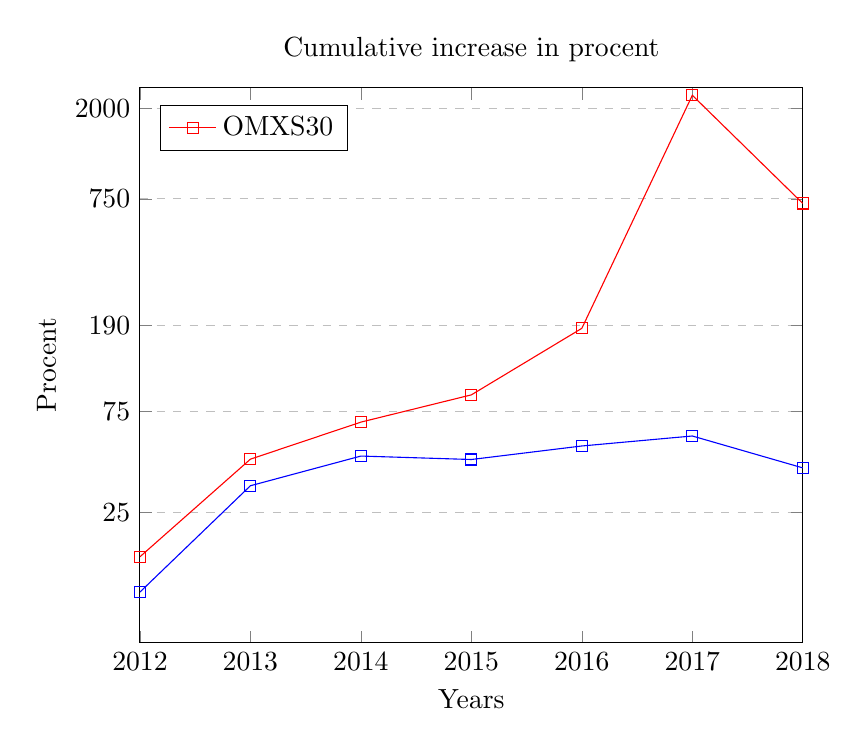
\begin{tikzpicture}
	\begin{axis}[    
	ymode=log,
	log ticks with fixed point,
	title={Cumulative increase in procent},
	xlabel={Years},
	ylabel={Procent},
	xmin=2012, xmax=2018,
	ymin=0, ymax=2500,
	xtick={2012,2013,2014,2015,2016,2017,2018},
	ytick={0,25,75,190,750,2000},
	legend pos=north west,
	ymajorgrids=true,
	grid style=dashed,
	/pgf/number format/.cd,
	use comma,
	1000 sep={}
	]
	
	\addplot[
	color=red,
	mark=square,
	]
	coordinates { % LAST + 100 * new percent = NEW
		(2012,15.44)(2013,44.52)(2014,66.55)(2015,89.44)(2016,184.08)(2017,2307)(2018,713.56)
	};
	\legend{Portfolio}
	
	\addplot[
	color=blue,
	mark=square,
	]
	coordinates {
		(2012,10.53)(2013,33.37)(2014,46.05)(2015,44.36)(2016,51.37)(2017,57.25)(2018,40.5)
	};
	\legend{OMXS30}
	
	\end{axis}
	
	\end{tikzpicture} \\
	* (1) Cryptocurrencies aren't included before 2016 since it wasn't a direct investment with high uncertainties of the exact numbers. \\
	* (2) Unlisted assets aren't included since there is no market to determine growth. In December 2017 most of these assets where made tradable and included from 1 Jan 2018. \\
	\\
	
	\subsubsection{Cryptocurrencies}
	\begin{tabular}{l|c|c|c|c|c|c|c}
		Currency & ICV YS & SEK YS & W. YS & ICV YE & SEK YE & W. YE & Procent \\
		bitcoin & \_ & 112,848 & 90,1 & \_ & 33,173 & 94,2 & \textcolor{red}{-70.7\%} \\
		ethereum & \_ & 6,163 & 6,4 & \_ & 1,180 & 4,4 & \textcolor{red}{-80,8\%} \\
		bitcoin cash & \_ & 19,911 & 3,3 & \_ & 1,438 & 0,9 & \textcolor{red}{-92.8\%} \\
		bitcoin sv & - & - & - & \_ & 754 & 0,4 & $ \infty $ \\
		ZCash & \_ & 4,145 & 0.06 & \_ & 497 & 0 & \textcolor{red}{-88\%} \\
		Total & - & \_ & 100 & - & \_ & 100 & \textcolor{red}{-72\%} 
	\end{tabular}\\
	\\
	
	% btc 80,544
	% eth 3,783
	% cash 732
	% sv 384
	% z 24.85
	% tot 85,467
	\subsubsection{Regulated markets}
	
	\begin{tabular}{l|c|c|c|c|c|c|c}
		Asset & shrs YS & SEK YS & W YS& shrs YE & SEK YE & W. YE & procent \\
		Tesla & \_ & 2,553 & 53.6 & \_ & 3,005 & ? & +17.7 \\
		Dometic & \_ & 83.55 & 5.7 & \_ & 53.85 & ? & -35.5 \\
		Fastout & \_ & 0.58 & 0.9 & \_ & 0.190 & ? & -67.2 \\
		LeoVegas & \_ & 83.75 & 8.8 & \_ & 41.40 & ? & -50.50 \\
		Marine harvest & \_ & 139 & 5.8 & \_ & 184.9 & ? & +33.0\\
		Raysearch & \_ & 171 & 4.49 & \_ & 97.45 & ? & -43.1\\
		
		Swedish crown & - & \_ & 20.6 & - & \_ & ? & -\% \\
		Inflow & - & \_ & 0 & 0 & - & - & - \\ 
		Total & - & \_ & - & - & \_ & 100 & \textcolor{green}{+3.98\%}
	\end{tabular} \\
	\\
	
	* As of 2018 inflow is completely unaccounted for, this for ease in counting. This would over time give a lower number than the real. The total is accounted for though as it's given in the nordnet analysis tool.
	
	\subsubsection{Unlisted}
	\begin{tabular}{l|c|c|c}
		Asset & shrs YS & SEK YS & W \\
		Kronfönster & \_ & 0 & 0 \\ 
		Barista & \_ & 0 & 0 \\
		Naava & \_ & 43 & 56.6 \\ %3526
		Pensiono & \_ & 50 & 43.4\\ %2700
		
		total & - & \_ & 100
	\end{tabular} \\
	\\
	\subsection{Total}
	\begin{tabular}{l|c|c|c|c|c}
		Asset Group & SEK YS & W YS & SEK YE & W. YE & procent \\
		Cryptocurrencies  & \_ & 92  & \_ & ? & $ \phi $ \\
		Regulated markets & \_  & 5.7 & \_  & ? & ? \\
		Unlisted          & \_   & 2.2 & \_   & ? & \textcolor{red}{-14,2\%}  \\
		Total             & \_   & 100 & ?   & \_ & \textcolor{red}{-66,2\%} \\
	\end{tabular}
	
	Notes: \\
	Coin prices from coinmarketcap for end 2018, for beginning see 2017 report. \\
	
	%bitcoin: 3737
	%etherium: 133
	%bicoin cash: 162
	%bitcoin sv: 85
	%zcash: 56
	
	31 dec: USD / SEK pair from exchange-rates.org. 8.8770 SEK \\
	
	\subsection{Output}
	
	As mentioned earlier this was a heavy year of work.
	
	\subsection{ITS}
	
	The 7 weeks at ITS was brutal as we didn't really get a proper assignment or any instructions whatsoever.
	I can't really be asked to more than I did although it feels a bit as a failure. Still I learned a bit more
	Java, and how to deal with an impossible task around people who didn't care or wanted to listen to reason.
	
	\subsubsection{Tremory}
	
	If you only look at the time committed, I must have looked like a super hero. There are a lot of stuff I maybe should address here but
	it still hurts a bit to think about. A lot of experiences transpired though and quite a few lessons where learned which otherwise are really hard to experience. The whole Uminova ordeal, renting Elasticys office, dealing with people developing under my lead and so on. 
	\subsubsection{Johnstedt.se}
	
	Didn't really do much with this site, published 2017s PDF and another over the n-queens report during the parallel course.
	
	\subsection{Personal Experience}
	
	This could possibly be left completely blanc as Eindhoven could be placed in either Output or Academic.
	
	\subsubsection{Eindhoven}
	
	I had the opportunity to visit Eindhoven as we won the local programmerings SM in umeå with CJ and Jakob. As Jakob was to old to compete in the regional competition Viktor went instead. 
	
	Maybe flashy for the CV and maybe a bit too fancy a competition. It is like math, people believe they can't do it so they won't even try. It retrieved in me some forgotten inner love for abstract problem solving, which incidentally have come to great use during my master thesis(as of this writing). 
	
\end{document}
